\section{Parameter survey, long crossovers, and update timing}
\label{sec:sline}

\subsection{Phase diagram}
\label{sec:sphase}

Figure~\ref{M-fig:phase} shows the surveyed invasion boundary $\qs(p)$ from strip fronts at $\alpha = 1/2$,
together with the interface density of the active phase just above it. The line is nonmonotonic.
The directly simulated D\&N reference has $\qs(0)\approx0.0184$; the line
rises steeply at small positive $p$ (0.0207 already at $p = 0.01$)
to a maximum of $\approx 0.049$ near $p = 0.25$--$0.5$ and then approaches the voter
point approximately as $\qs\approx 0.25\,\alpha(1-p)$ over the sampled range
(Table~\ref{tab:line}). The initial rise is consistent with the voter
moves at $j = 4,5$, which D\&N forbids and which smooth interfaces.
The broad parameter survey finds sign-changing strip velocities and apparent
bulk plateaus $\rho_+ = 0.23$--$0.32$ at its stated observation times
[Fig.~\ref{M-fig:phase}(b)]. These finite-window densities do not determine the
limiting jump as $p\to1$. No tricritical point is resolved on this grid;
the longer-time assessment in Sec.~\ref{M-sec:voter} is essential near the endpoint.

\begin{table}
\caption{Broad finite-time survey at $\alpha=1/2$. Invasion thresholds
$\qs$ come from strip fronts (usually $L_x=2048$, $L_y=4096$, $T=10^5$,
2--4 seeds; $p=0$: five runs per probability across $L_x=2048,8192$;
$p\ge0.99$: note $b$), except for the refined $p=1/2$
estimate in Sec.~\ref{M-sec:fronts}. The bulk column gives the actual probability
$q_\rho$ and apparent plateau density $\rho_+$, using all selected runs at
$L\ge2048$ and time integration per run ($T\ge10^5$;
$p\ge0.98$: $T=10^6$--$1.5\times10^6$).
$c=\qs/[\alpha(1-p)]$. These densities are finite-window measurements.}
\label{tab:line}
\begin{ruledtabular}
\begin{tabular}{lllll}
$p$ & $\qs$ & $q_\rho$ & $\rho_+$ & $c$ \\
\hline
$0^{\,a}$ & 0.01837 & 0.0185 & 0.226 & -- \\
0.01 & 0.02070 & 0.021 & 0.245 & 0.042 \\
0.02 & 0.02280 & 0.02332 & 0.256 & 0.047 \\
0.05 & 0.02874 & 0.029 & 0.257 & 0.061 \\
0.1 & 0.03680 & 0.037904 & 0.288 & 0.082 \\
0.25 & 0.04932 & 0.05047 & 0.307 & 0.132 \\
0.5 & 0.04594 & 0.046359 & 0.302 & 0.184 \\
0.75 & 0.0276 & 0.0286 & 0.316 & 0.221 \\
0.9 & 0.01194 & 0.0122 & 0.290 & 0.239 \\
0.95 & 0.00619 & 0.0065 & 0.289 & 0.248 \\
0.98 & 0.00252 & 0.0025704 & 0.260 & 0.252 \\
0.99$^{\,b}$ & 0.00128 & 0.00128$^{b}$ & 0.241 & 0.256 \\
0.995$^{\,b}$ & 0.00064 & 0.00064$^{b}$ & 0.234 & 0.256 \\
\end{tabular}
\end{ruledtabular}
\begin{flushleft}\footnotesize
$^{a}$Direct $p=0$ reference, where the model has additional frozen configurations
(Supplemental Sec.~\ref{app:frozen}).\\
$^{b}$Runs of $1.2\times10^6$ ($p = 0.99$) and $1.6\times10^6$ steps ($p = 0.995$), four times the
crossover time $t_\times$ of Sec.~\ref{M-sec:voter}, four seeds, velocities fitted for $t\ge t_\times$
from the strip profile (Supplemental Sec.~\ref{app:numerics}); from runs of $10^5$ steps the
crossing at $p = 0.995$ is 0.00062 (Sec.~\ref{M-sec:voter}).
The bulk averages combine the nearby probabilities 0.00128 and 0.0012827 at
$p=0.99$, and 0.00064 and 0.0006417 at $p=0.995$; these are descriptive
survey values, not a limiting-density extrapolation. Their pooled standard
errors describe variation across these nearby parameters and horizons.
The new $2\times10^7$-step runs at $p=0.995$, $q=0.000640$ show
continuing decay (Sec.~\ref{M-sec:voter}); the tabulated threshold and density
there are historical finite-window estimates.
\end{flushleft}
\end{table}



\subsection{Near the voter point}
\label{sec:svoter}

As $p\to 1$ the transition approaches the voter point, where logarithmic corrections make every
diagnostic slow. A finite-window fit to one voter-model run at $L=4096$
gives $1/\rho\simeq0.184\ln t+2.13$ over $10^3\le t\le10^6$;
its slope depends on the fit start and is not an asymptotic amplitude.
A density that looks stationary over a finite window is therefore not enough.
We compare four complementary diagnostics at $p = 0.98$,
$0.99$, and $0.995$, with the noise strength measured by $\delta = q/\qs - 1$.

\textit{Bulk relaxation and front drift.} The earlier survey found apparent
plateaus $\rho\approx0.23$--$0.26$ over $10^6$--$1.5\times10^6$ steps at
$L=2048$ and 4096, including points very close to its estimated invasion
boundary. The sensitivity of that boundary to observation time already
signaled a long crossover. At $p=0.995$, a $10^5$-step strip estimate gives
$q\approx0.00062$, where the bulk subsequently decays; extending the strips
to $1.6\times10^6$ steps moves the crossing to approximately $0.000640$,
with a quoted spread of $5\times10^{-6}$ across the earlier estimates.
The analogous $1.2\times10^6$-step estimate at $p=0.99$ is about $0.00128$.
Table~\ref{tab:line} records this finite-time survey. Agreement between two
sizes over that horizon does not establish stationarity at longer times.
At $p=0.99$ the apparent plateau decreases on approaching the boundary:
$1/\rho$ changes from 3.60 at $q\approx1.19\,\qs$ to 4.11 near $\qs$.
These finite-window values alone distinguish neither a small limiting jump
nor logarithmically slow continuous vanishing.

The longer fixed ensembles at $p=0.995$ expose the limitation directly
(Fig.~\ref{fig:gpu_near}). At $L=4096$, the four-run mean density at
$q=0.000636$ falls from 0.201 over $10^6$--$2\times10^6$ steps to
0.027 over $5\times10^6$--$10^7$; all four runs reach consensus by
$10^7$. At $q=0.000640$, none reaches consensus by that time, but the
successive window means decrease from 0.228 to 0.216 to 0.207. At
$q=0.000644$ and 0.000648, the late means are 0.229 and 0.233 and no
late drift is resolved within the four-run uncertainty. These observations
separate collapse from persistence over a substantially longer horizon,
without identifying the limiting order parameter at the boundary.

Extending $L=8192$ runs to $2\times10^7$ steps makes the drift at
$q=0.000640$ clearer. The four-run mean falls from 0.189 over
$5\times10^6$--$10^7$ to 0.122 over $10^7$--$2\times10^7$,
with a 95\% run-bootstrap interval $[0.078,0.168]$ for the latter, and
one run reaches consensus. The difference between the second and first
halves of that window is $-0.055$, with interval $[-0.092,-0.027]$.
The earlier apparent plateau at this probability is therefore not a
stationary active-state measurement.
An independent midpoint ensemble at $q=0.000642$ retains activity in all
four runs, with late mean 0.2204 and interval $[0.2159,0.2231]$.
All four midpoint runs have a negative within-window change: $-0.0046$ with
interval $[-0.0077,-0.0015]$, about 2.1\% of its late mean. A paired $t_3$ reference interval is
$[-0.0109,+0.0016]$; the percentile interval has limited coverage accuracy
with four runs. We report the individual changes in Fig.~\ref{M-fig:gpu_near20m}
and do not assign a method-independent significance to the mean drift.
At $q=0.000644$ and 0.000648, all four $L=8192$ runs remain active
through $2\times10^7$, with late means 0.2265 and 0.2326 and no resolved
drift within $10^7$--$2\times10^7$. This separates late decay from
persistence on the sampled grid; bulk persistence alone still does not
locate an asymptotic coexistence boundary.
Figure~\ref{M-fig:gpu_near20m} shows the full largest-system time traces
and their paired late-window changes.

The strip experiment has a related limitation. At $q=0.000640$, activity
within the initial strip interior decays strongly and only one of four
runs retains valid separated-front geometry throughout
$5\times10^6\le t\le10^7$. An envelope fitted to the fragmented band
would mix front motion with internal decay. We therefore do not assign
a stationary front velocity to that ensemble. At higher $q$ the interior
persists, but expanding bands can instead encounter the finite box.
Both failures are visible in the width and interior-activity diagnostics.

\begin{figure*}
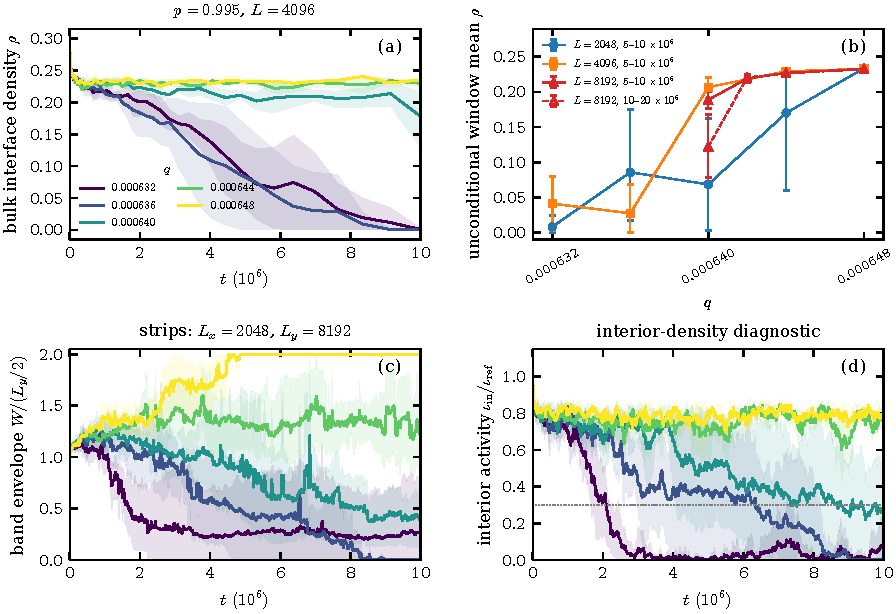
\includegraphics[width=\textwidth]{figs/fig_gpu_near}
\caption{Long-time tests near the voter point, $p=0.995$, $\alpha=1/2$;
four independent runs per parameter set. Colors in (a,c,d) denote the same $q$.
(a) Bulk density at $L=4096$ to $10^7$ steps.
(b) Unconditional time-weighted bulk means over the common
$5\times10^6\le t\le10^7$ window at three sizes, together with the later
$10^7$--$2\times10^7$ window at $L=8192$.
(c) Outer-envelope width of initially half-filled active strips,
$L_x=2048$, $L_y=8192$, normalized by the initial half-box width.
(d) Activity in the initial central interior region, relative to its
reference value at $t=10^3$. The dotted line is the profile threshold used
for the envelope. A changing interior density must be distinguished from
motion of a stationary front. Bands and bars are pointwise 95\%
run-bootstrap intervals. Absorbed trajectories are extended by their known
zero activity, and only complete predeclared seed ensembles are shown.}
\label{fig:gpu_near}
\end{figure*}



\textit{Size dependence of the magnetic fluctuations.} A split into an Ising
and a DP transition would leave an ordered active window. At the Ising point,
$\chi_L=L^2\langle m^2\rangle\sim L^{7/4}$, giving
$\chi_{4096}/\chi_{2048}=2^{7/4}\simeq3.36$.
Unfiltered, time-weighted run estimates show much weaker size dependence
at several sampled active points [Fig.~\ref{fig:voter}(a)]. For example,
at $p=0.98$, $q=0.0025704$, the ratio is $1.09$ with a pointwise
95\% run-bootstrap interval $[0.82,1.52]$.
Closer to the endpoint and threshold the uncertainty is larger:
at $p=0.99$, $q=0.0012827$, the ratio is $0.92$ with interval
$[0.34,4.20]$, and at $p=0.995$, $q=0.000651$, it is $1.95$
with interval $[1.07,3.46]$. These latter intervals include the Ising
size factor; restricting both sizes to the common window
$2\times10^5\le t\le5\times10^5$ leaves similarly large uncertainty.
No ordered active interval is resolved by the present grid,
but these measurements cannot exclude a narrower interval near the boundary.
The new $p=0.995$ ensembles at $q=0.000648$ give
$\chi_{4096}/\chi_{2048}=1.18$ with interval $[0.72,1.98]$ over the
common $5\times10^6$--$10^7$ window; all four runs at each size remain
active. This constrains fluctuations at that sampled active point.
The further doubling gives $\chi_{8192}/\chi_{4096}=0.91$ with interval
$[0.48,1.70]$ over the same window, also without absorption.
Closer to the boundary, absorption in the smaller systems contributes
$m^2=1$ and prevents interpreting an unconditioned size ratio as an
equilibrium critical-scaling test.

\textit{Suppression of small seeds.} A $2\times2$ block of live sites in the dead state
spreads, in the voter model, with survival probability $P_s(t)\simeq A\ln t/t$~\cite{bramson1980},
i.e., a local exponent $\delta_{\rm eff} = -\ds\ln P_s/\ds\ln t$ approaching 1 from below. GV criticality has voter-like asymptotic spreading, but this does not impose a finite-time bound on $\delta_{\rm eff}$ in a nonlinear model~\cite{castellano2012,azizi2020}; at a DP point $\delta_{\rm eff}\to0.451$. Figure~\ref{fig:voter}(b)
shows $t\,P_s(t)$, which grows as $\ln t$ for the voter model. At sampled
nonlinear-model points where the bulk remains active over the observation
window, this quantity instead decreases over substantial intervals.
The contrast is consistent with a nucleation barrier to invasion from
small seeds. At $p=0.99$, $q=0.0012954$, an independent predeclared
ensemble of $8\times10^6$ seeds leaves 19 survivors and no escapes at
$t=10^6$. Thus $P_s=2.375\times10^{-6}$, with an exact two-sided 95\%
binomial interval $[1.430,3.709]\times10^{-6}$. All sixteen fixed-size
shards of 500000 replicas completed with adaptive stopping disabled.
Between $t_1=63096$ and $t_2=251189$, the survival count falls from
793 to 97. The approximately factor-four-window estimate
$\delta_{\rm eff}=-\ln[P_s(t_2)/P_s(t_1)]/\ln(t_2/t_1)$ is 1.52,
with a pointwise 95\% conditional-binomial interval $[1.39,1.66]$.
The decay slope does not keep increasing: the last supported factor-four
window, $t=223872$--891251, gives 1.26 with interval $[0.99,1.59]$.
No terminal slope is quoted because 19 survivors fall below the
predeclared minimum count of 20. Overlapping windows are correlated
and are not fitted as independent exponent estimates. These observations
quantify intermediate-time seed suppression while leaving the asymptotic
survival probability and critical scaling unresolved.
At $p=0.995$, $q=0.0006324$, below the estimated threshold, none of
$3\times10^6$ seeds survives to $10^6$. Further above threshold the seeds
overshoot and then level off: at $p=0.99$, $q=0.0013335$, running to
$t=10^6$ on $L=8192$ gives 40 recorded survivors or escapes, compared with
88 at $10^5$. One of the terminal replicas has escaped, so the observed
late-retention ratio is bounded by $39/88$ and $40/88$, approximately
$0.44$--$0.45$, before sampling uncertainty; the voter asymptote gives
about 0.12. These higher-$q$ shards stopped at survivor targets, with
750839 replicas in total. Their curves are descriptive finite-time
evidence of slower late decay, and neither their stopping protocol nor
their observation horizon identifies a limiting survival probability.

\textit{Walls are wetted below the threshold.} A flat wall between the two absorbing phases
(protocol v) roughens like a voter interface at first, $W\propto t^{1/2}$, independent of $q$. After
a crossover time $t_\times$, $q$ takes over (Fig.~\ref{fig:voter}(c)). Below $\qs$ ($\delta =
-0.02$ at $p\le 0.98$, $-0.03$ at $0.99$, $-0.05$ at $0.995$) the wall turns into a slab of the
active phase with a long-lived finite width, $W(10^6)\approx 200$,
450, 670, and 820 for $p = 0.9$, 0.98, 0.99, 0.995, whose interior has an interface-site
fraction of 0.46--0.51, comparable to the earlier finite-window bulk estimates
near reversal (0.47--0.58); the pure voter wall
keeps widening. Above
$\qs$ the slab edges move outward at the strip-front velocities.
The crossover time increases from $\approx10^4$ at $p=0.9$ to
$\approx4\times10^5$ at $p=0.995$; the sampled-range fit
$t_\times\propto(1-p)^{-1.3}$ is an effective description, not an
asymptotic scaling law. This initial crossover marks the time at which
the perturbation becomes visible. The new longer runs show that it need
not mark final relaxation: the transition order remains unresolved at
$p=0.995$ and closer to the voter point.

These measurements follow the invasion boundary toward the voter point
and provide finite-time diagnostics of possible continuation of discontinuous behavior.
They do not establish that continuation at $p=0.995$, where threshold
uncertainty and relaxation times are largest. Accelerated seed extinction
supports a nucleation interpretation, rather than a universal finite-time
test excluding GV criticality. We distinguish these endpoint results from
the well-resolved coexistence at $p=1/2$ and from a claim about every fixed
$p<1$.

\begin{figure*}
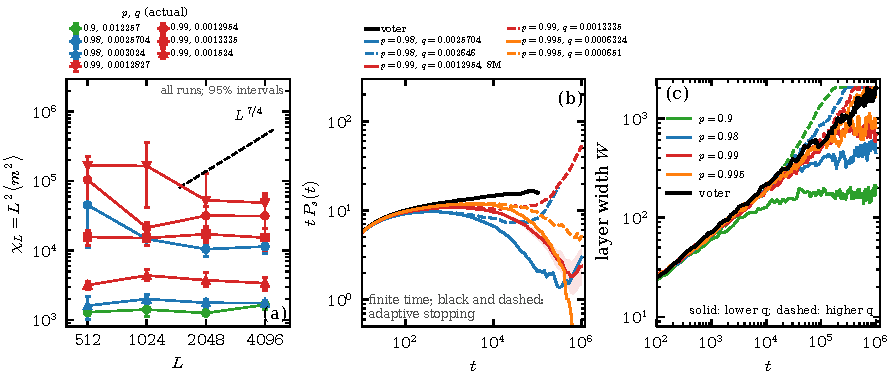
\includegraphics[width=\textwidth]{figs/fig_voter}
\caption{Near the voter point. (a) Unconditioned magnetic second moment
$\chi_L = L^2\langle m^2\rangle$ from random starts for $p=0.9$, 0.98,
and 0.99; the legend gives actual $q$. Each point averages 2--8 independent
runs after time integration over $t\ge2\times10^5$, with final times
$5\times10^5$ or $10^6$. Bars are pointwise 95\% run-bootstrap intervals.
No activity filter is applied: trajectories reaching consensus contribute
$m^2=1$ thereafter, which affects the small systems. The dashed line is
the Ising law $L^{7/4}$. (b) Survival of a $2\times2$ seed in
the dead state, $t\,P_s(t)$, which grows as $\ln t$ for the voter model (black, $L = 2048$), decays
when small seeds are strongly suppressed, and would grow linearly for a
positive limiting survival probability. The red solid curve at $p=0.99$,
$q=0.0012954$ uses the complete independent fixed-$N$ ensemble of
$8\times10^6$ replicas. Shading gives pointwise 95\% binomial intervals
(Clopper--Pearson for sparse counts, Wilson otherwise). Other nonlinear
solid curves retain the earlier $3\times10^6$-replica ensembles.
The black voter reference and higher-$q$ dashed curves use adaptive
survivor-target stopping and are shown descriptively.
The black reference stops at 300 retained replicas out of 1,905,766,
including 11 escapes at $t=10^5$; its plotted retained fraction is the upper
survival bound. Lattice size is
$L=8192$ for the nonlinear models; escapes are recorded separately.
(c) Width $W$ of the active
layer on a flat wall between the two absorbing phases, $L_x=1024$, $L_y=4096$,
two seeds. The pairs of lower (solid) and higher (dashed) probabilities are
$(0.011662,0.012495)$, $(0.0024696,0.002646)$,
$(0.0012446,0.0013335)$, and $(0.0006076,0.000651)$ for
$p=0.9$, 0.98, 0.99, and 0.995, respectively. Black: the voter model
($p=1$, $q=0$).}
\label{fig:voter}
\end{figure*}

\subsection{Synchronicity and asynchronous updating}
\label{sec:async}

The D\&N weight $\alpha$ sets the scale of $\qs$. Near the voter point the measured threshold is consistent with proportionality to $\alpha$: strip fronts at $\alpha = 1/4$, $1/2$, and 1 for $p = 0.98$ and 0.99 give
$\qs\propto\alpha^{\beta}$ with $\beta = 1.00\pm0.02$ and $c = \qs/[\alpha(1-p)] = 0.248$--$0.258$
(Table~\ref{tab:alpha}), consistent with the finite-time closure of
Sec.~\ref{M-sec:theory}. At the directly simulated $p=0$ reference, the
finite-density branch persists at the sampled $\alpha$ values between $1/8$
and 1, with no tricritical point resolved on that grid.

To test sensitivity to parallel updating, we make the dynamics lazy: each site
is updated with probability $r$ per step (the flip table is multiplied
by $r$), so $r\to 0$ is continuous time and $rt$ is the physical time. At $p = 0.98$ the front
velocity still changes sign. Nominal linear fits give
$\qs(r)/\qs(1) = 0.864\pm0.010$, $0.858\pm0.016$,
and $0.870\pm0.012$ for $r = 1/2$, $1/4$, and $1/8$.
These legacy fits use selected profile windows and extrapolate slightly
beyond their fitted probability range. Alternative documented fit ranges
shift the ratios by as much as 0.05, beyond the quoted sampling errors.
No monotonic change among the sampled $r\le1/2$ is resolved within that
systematic variation. At
$p = 0.99$, $r = 1/4$, fronts just above $\qs(r)$ retreat for $\sim 10^5$ physical time units
before advancing, and the late-time crossing, $0.85$--$0.88$, agrees with $p = 0.98$. At the
representative point $p=1/2$, corrected outer-envelope tracking of three
strips over physical times $2.5\times10^4$--$5\times10^4$ gives a
finite-window crossing $q^*(1/4)\simeq0.03963$, or roughly 0.86 of the
synchronous value. Earlier windows and profile thresholds produce shifts
of several $10^{-3}$ in this ratio, so greater asymptotic precision is
not assigned. The bulk active phase at $q=0.040392$ has a late-window mean
$\rho\simeq0.2105$ through physical time $10^5$, while at $q=0.039474$
it decays slowly. Supporting near-voter runs show bulk plateaus over a
factor 40 in time at roughly 10\% above the nominal crossing, early seed
decay with $\delta_{\rm eff}>1$, and active wall layers below the nominal
crossing while the lazy-voter wall keeps widening. The legacy seed curves
use adaptive stopping, and boundary escapes contaminate their late retained
counts, so no survival plateau is inferred from them.
These finite-$r$ checks show robustness to reduced update probabilities.
Establishing the strict continuous-time transition requires an extrapolation
in $r$.

\begin{table}
\caption{Synchronicity and asynchrony near the voter point. Top: $\qs\propto\alpha$ (strip
fronts, four seeds; errors are seed bootstrap, systematic $\approx\pm2\%$). Bottom: lazy updating
with probability $r$ per step at $p = 0.98$ and $1/2$; $c(r)$ from simulation and, near the voter
point, from the theory of Sec.~\ref{M-sec:theory}. The $p=0.98$ bottom entries
are nominal finite-window, profile-selected estimates; parentheses give
sampling errors, while probability-fit-range changes shift their ratios
by up to 0.05. The $p=1/2$ entry uses the corrected envelope over physical
times $2.5\times10^4$--$5\times10^4$ and is rounded to reflect window and
threshold sensitivity. Theory entries use fixed dual time $T=65536$
for synchronous walks and physical dual time $rT=65536$ for lazy walks;
their parentheses include walk-sampling uncertainty only.}
\label{tab:alpha}
\begin{ruledtabular}
\begin{tabular}{lllll}
$p$ & $\alpha$ & $\qs$ & $c$ (sim.) & $c$ (theory) \\
\hline
0.98 & 0.25 & 0.001274(9) & 0.255 & \\
0.98 & 0.5 & 0.002515(19) & 0.252 & \\
0.98 & 1 & 0.005074(30) & 0.254 & 0.255(2) \\
0.99 & 0.25 & 0.000621(18) & 0.248 & \\
0.99 & 0.5 & 0.001292(7) & 0.258 & \\
0.99 & 1 & 0.002553(9) & 0.255 & \\
\hline
$p$ & $r$ & $\qs(r)/\qs(1)$ & $c(r)$ (sim.) & $c(r)$ (theory) \\
\hline
0.98 & 1/2 & 0.864(10) & 0.218 & 0.221(3) \\
0.98 & 1/4 & 0.858(16) & 0.216 & 0.206(4) \\
0.98 & 1/8 & 0.870(12) & 0.219 & 0.200(4) \\
0.5 & 1/4 & $\approx0.86$ & 0.159 & -- \\
\end{tabular}
\end{ruledtabular}
\end{table}

%=====================================================================================
